%%%%%%%%%%%%%%%%%%%%%%%%%%%%%%%%%%%%

\section{4.2. Intervalos de confiança}

%%%%%%%%%%%%%%%%%%%%%%%%%%%%%%%%%%%%

\subsection{Por que relatamos intervalos de confiança?}

%%%%%%%%%%%%%%%%%%%%%%%%%%%%%%%%%%%%

\begin{frame}
\frametitle{Intervalos de confiança}
\footnotesize
\begin{itemize}
\justifying
\item Um intervalo de valores plausível para um parâmetro da população é chamado de \hl{intervalo de confiança}.
\justifying
\item Usar apenas uma estatística de amostra para estimar um parâmetro é como pescar em um lago escuro com uma lança, mas usar um intervalo de confiança é como pescar com uma rede.
$\:$ \\
$\:$ \\
\begin{columns}[c]
\column{0.25\textwidth}

\includegraphics[width=\textwidth]{4-2_conf_int/spear.jpg}
\column{0.5\textwidth}
\justifying
{\footnotesize
Podemos jogar uma lança onde vimos um peixe, mas provavelmente o perderemos. Se atirarmos uma rede nessa área, temos uma boa chance de pegar o peixe.
}
\column{0.25\textwidth}

\includegraphics[width=\textwidth]{4-2_conf_int/net.jpg}
\end{columns}
$\:$ \\

\item Se utilizarmos apenas uma estimativa pontual, provavelmente não atingiremos o parâmetro populacional exato. Se utilizarmos um intervalo de valores plausíveis, temos uma boa chance de alçancar o parâmetro.

\end{itemize}

{\tiny Photos by Mark Fischer (http://www.flickr.com/photos/fischerfotos/7439791462) and Chris Penny (http://www.flickr.com/photos/clearlydived/7029109617) on Flickr.}\\

\end{frame}


%%%%%%%%%%%%%%%%%%%%%%%%%%%%%%%%%%%%

\subsection{Construindo um intervalo de confiança}

%%%%%%%%%%%%%%%%%%%%%%%%%%%%%%%%%%%%

\begin{frame}
\frametitle{Número médio de relacionamentos exclusivos}
\justifying
\dq{Uma amostra aleatória de 50 estudantes universitários foi questionada sobre quantos relacionamentos exclusivos eles mantinham até então. Esta amostra rendeu uma média de 3,2 e um desvio padrão de 1,74. Estime o verdadeiro número médio de relacionamentos exclusivos usando essa amostra.}

\pause 

\vspace{-0.5cm}
\[ \bar{x} = 3.2 \qquad s = 1.74 \]

\pause
\justifying
O intervalo de confiança aproximado de 95\% é definido como
\[ estimativa ~ pontual \pm 2 \times SE \]

\pause

\vspace{-0.25cm}
\[ SE = \frac{s}{\sqrt{n}} = \frac{1.74}{\sqrt{50}} \approx 0.25 \]

\end{frame}

%%%%%%%%%%%%%%%%%%%%%%%%%%%%%%%%%%%%%%%%%%%

\begin{frame}
\frametitle{Número médio de relacionamentos exclusivos}

\vspace{-0.25cm}
\begin{eqnarray*}
\bar{x} \pm 2 \times SE &=& 3.2 \pm 2 \times 0.25 \\
\pause
&=& (3.2 - 0.5, 3.2 + 0.5) \\
\pause
&=& (2.7, 3.7)
\end{eqnarray*}


\end{frame}

%%%%%%%%%%%%%%%%%%%%%%%%%%%%%%%%%%%

\begin{frame}
\frametitle{Prática}
\justifying
\pq{Qual das seguintes interpretações deste intervalo de confiança é a correta?}
\justifying
Estamos 95\% confiantes de que
\begin{enumerate}[(a)]
\justifying
\item o número médio de relacionamentos exclusivos que os estudantes universitários da amostra estiveram é entre 2,7 e 3,7.
\justifying
\solnMult{Em média, os estudantes universitários têm entre 2,7 e 3,7 relacionamentos exclusivos.}
\justifying
\item um estudante universitário escolhido aleatoriamente tem de 2,7 a 3,7 relacionamentos exclusivos.
\justifying
\item 95\% dos estudantes universitários têm de 2,7 a 3,7 relacionamentos exclusivos.
\end{enumerate}

\end{frame}

%%%%%%%%%%%%%%%%%%%%%%%%%%%%%%%%%%%

\subsection{Um intervalo mais preciso}

%%%%%%%%%%%%%%%%%%%%%%%%%%%%%%%%%%%

\begin{frame}
\frametitle{Um intervalo mais preciso}
\justifying
\formula{Intervalo de confiança, uma fórmula geral}
{\[ estimativa ~ pontual \pm z^\star \times SE \] }

\pause
\justifying
Condições para ter uma estimação pontual = $\bar{x}$:
\begin{enumerate}
\justifying
\item \hlGr{Independência:} As observações na amostra devem ser independentes
\begin{itemize}
\justifying
\item amostragem/atribuição aleatória
\justifying
\item se amostragem sem reposição, $n <$ 10\% da população
\end{itemize}
\justifying
\item \hlGr{Tamanho da amostra/assimetria:} $ n \ge 30 $ e a distribuição da população não deve ser extremamente assimétrica.

\end{enumerate}

$\:$ \\
\pause
\justifying
{\tiny
\orange{Nota:} Vamos discutir sobre amostras onde $ n <30 $ no próximo capítulo.}

\end{frame}

%%%%%%%%%%%%%%%%%%%%%%%%%%%%%%%%%%%%

\subsection{Capturando o parâmetro populacional}

%%%%%%%%%%%%%%%%%%%%%%%%%%%%%%%%%%%

\begin{frame}
\frametitle{O que significa 95\% de confiança?}

\begin{itemize}
\justifying
\item Suponha que tiramos muitas amostras e construímos um intervalo de confiança de cada amostra usando a equação: \\ {\[ estimativa ~ pontual \pm z^\star \times SE \] }
\justifying
\item Então, cerca de 95\% desses intervalos conteriam a média real da população ($\mu$). 

\end{itemize}

\twocol{0.5}{0.5}
{
\begin{itemize}
\justifying
\footnotesize
\item A figura mostra esse procedimento com 25 amostras, em que 24 dos intervalos de confiança resultantes contém o número médio real de relacionamentos exclusivos e um intervalo não contém o número médio real.

\end{itemize}
}
{
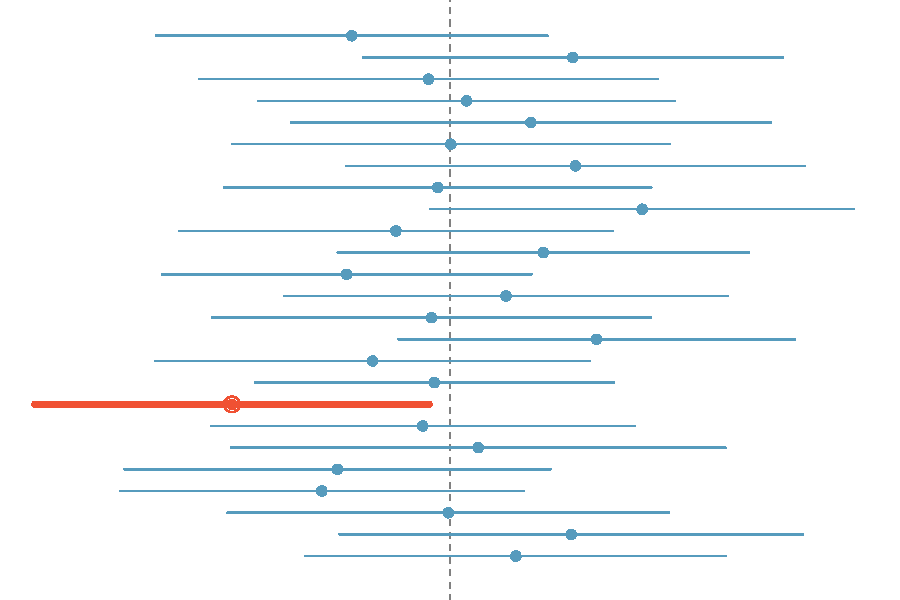
\includegraphics[width=\textwidth]{4-2_conf_int/95PercentConfidenceInterval.pdf}
}

\end{frame}

%%%%%%%%%%%%%%%%%%%%%%%%%%%%%%%%%%%

\begin{frame}
\frametitle{Largura de um intervalo}
\justifying
\dq{Se queremos ter mais certeza de que capturamos o parâmetro população, ou seja, se queremos aumentar o nosso nível de confiança, devemos usar um intervalo maior ou um intervalo menor?}

\pause

\soln{Um intervalo maior.}

$\:$ \\

\pause
\justifying
\dq{Você consegue ver alguma desvantagem em usar um intervalo maior?}
\begin{center}

\includegraphics[width=0.6\textwidth]{4-2_conf_int/garfield.png}
\end{center}

\pause
\justifying
\soln{Se o intervalo for muito largo, pode não ser muito informativo.}\\
\justifying
{\scriptsize Image source: http://web.as.uky.edu/statistics/users/earo227/misc/garfield\_weather.gif}

\end{frame}



%%%%%%%%%%%%%%%%%%%%%%%%%%%%%%%%%%%

\subsection{Alterando o nível de confiança}

%%%%%%%%%%%%%%%%%%%%%%%%%%%%%%%%%%%

\begin{frame}
\frametitle{Alterando o nível de confiança}
\justifying
\[ estimativa~pontual\pm z^\star \times SE \] 

\begin{itemize}
\justifying
\item Em um intervalo de confiança, $z ^ \star \times SE $ é chamado de \hl {margem de erro} e, para uma determinada amostra, a margem de erro é alterada conforme o nível de confiança é alterado.
\justifying
\item Para alterar o nível de confiança, precisamos ajustar $ z ^ \star $ na fórmula acima.
\justifying
\item Os níveis de confiança comumente usados são 90\%, 95\%, 98\% e 99\%.
\justifying
\item Para um intervalo de confiança de 95\%, $ z ^ \star = 1.96 $.
\justifying
\item No entanto, usando a distribuição normal padrão ($ z $), é possível encontrar o $ z ^ \star $ apropriado para qualquer nível de confiança.

\end{itemize}

\end{frame}

%%%%%%%%%%%%%%%%%%%%%%%%%%%%%%%%%%%%

\begin{frame}
\frametitle{Prática}
\justifying
\pq{Qual dos valores abaixo de Z é o $z ^ \star $ apropriado ao calcular um intervalo de confiança de 98\%?}

\begin{multicols}{2}
\begin{enumerate}[(a)]
\item $Z = 2.05$
\item $Z = 1.96$
\solnMult{$Z = 2.33$}
\item $Z = -2.33$
\item $Z = -1.65$
\item[]
\end{enumerate}
\end{multicols}


\begin{center}
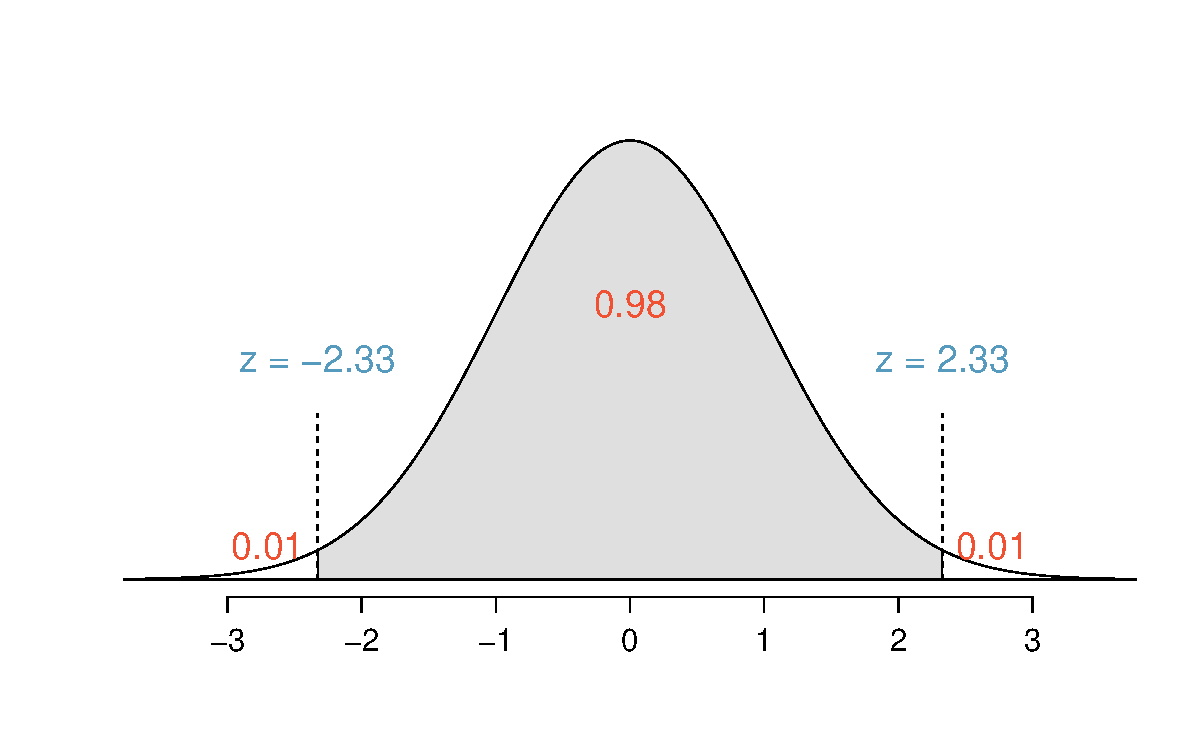
\includegraphics[width=0.7\textwidth]{4-2_conf_int/middle98.pdf}
\end{center}


\end{frame}

%%%%%%%%%%%%%%%%%%%%%%%%%%%%%%%%%%%

